% !TeX spellcheck = en_GB
\section{Observations at the weather mast}
\label{sec:loc_obs}
\textcolor{red}{If used here, then not in the weather situation, but keep the wind damage table.}
%The large scale synoptic analysis will be related to the local weather  observations at Haukeliseter. 
It is a primary goal of this work to relate the local weather observations from the WMO site at Haukeliseter to the synoptic scale structure and the additional measurements taken at Haukeliseter during the winter of 2016/2017.
\\
Examples of the \SI{60}{\minute} precipitation accumulation from the double fence rain gauge, \SI{2}{\metre} air temperature, and wind observations are presented in \Cref{fig:TPU} to document the continuous precipitation at Haukeliseter during the extreme event. 
 %%% local observations @ Haukeliseter %%%%%%%%%%%%%%%%%%%%%%%%%%%%%%%%%%%%%
 \begin{figure}[ht!]
 	\centering
 	%%%%%% 24/12
	\begin{subfigure}[b]{\textwidth}
		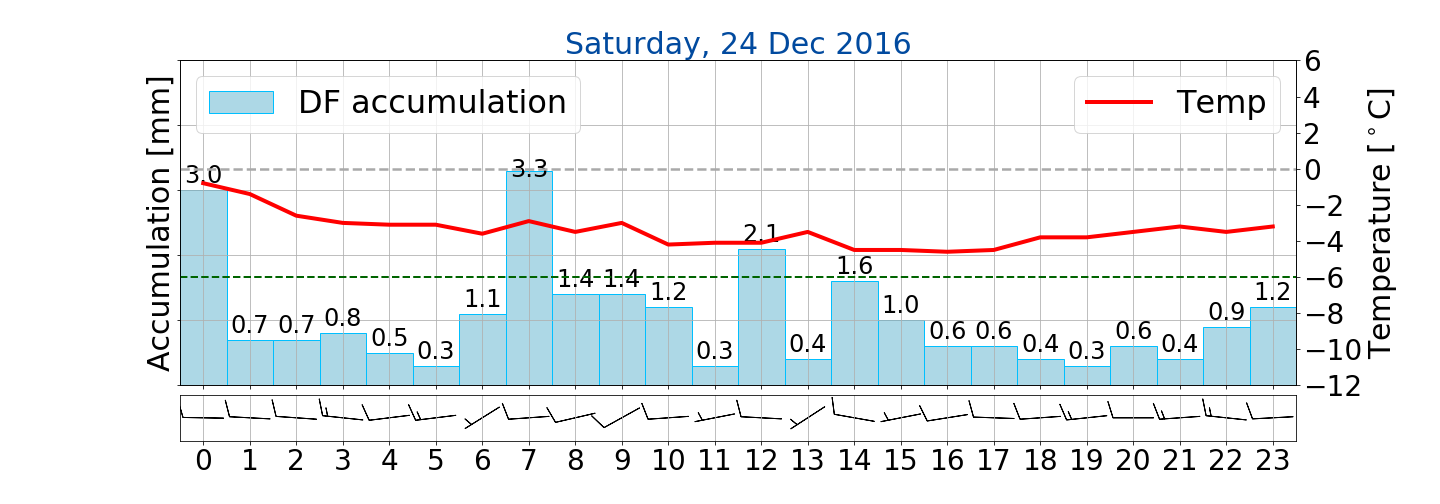
\includegraphics[trim={4.9cm 1.cm 1.5cm 1cm},clip,
		width=\textwidth]{./fig_weathermast/T_P_U_20161224}
		\caption{}\label{fig:TPU}
	\end{subfigure}
 \caption{Surface precipiation, temperature and wind observation from the weather mast at Haukeliseter on \SI{24}{\dec}. \SI{60}{\minute} total accumulation [\SI{}{\mm}] in light blue as bar, temperature (red, [\SI{}{\celsius}]), and wind as barbs [\SI{}{\mPs}]. Gray dashed line indicates the freezing temperature and the green dashed line the 30-year climate mean temperature at \SI{-6}{\celsius}. Hourly processed data taken from \cite{eklima_norwegian_2016}.} \label{fig:TPU}
 \end{figure}
 %%%%%%%%%%%%%%%%%%%%%%%%%%%%%%%%%%%%%%%%%%%%%%
\noindent
The temperature evolution will be used to investigate possible changes in the type of precipitation. 
\\
Snowfall is likely for temperatures up to \SI{2}{\celsius}. The intensity of the storm can be classified by the hourly averaged wind speed and direction as wind barbs in \SI{}{\mPs}.
To understand which damage a storm can have, \cite{faeraas_urd_2016} released a table to associate wind strength with damage (see \Cref{tab:wind}).
% \\
%%%%%%%%%%%%%%%%%%%%%%%%%
